\chapter{Introduction}
Historically, it was always assumed by cybersecurity experts that the hardware underlying information
systems were always secure and \textit{trusted}, but was it really the case? The answer is no, and 
this has some serious implications.\\ 
For example, the data can be considered secure while traveling trough a secure channel, but it is 
meaningless if the source of the destination isn't secure, both from a software and hardware perspective.\\
This means that the access point from which the data is extracted can actually be the hardware itself,
for example accessing the data directly from a register of using a side-channel attack.\\
But most importantly, while software issues can be patched with a simple update, hardware issues are
much more difficult to fix, because there are no easy ways to update the hardware: it is safe to 
assume that once a hardware vulnerability is discovered, it will be there forever.\\
The only actual "fix" is to replace the hardware, which is not always possible, especially if its 
very expensive or if it is embedded in a system, such as a satellite.\\
Alternatively, sometimes patches are rolled out to reduce the impact of the vulnerability, by reducing
the capability of exploiting it, but this is not always possible and never a definitive solution.\\

But first thing first, what we consider as hardware?\\
\begin{boxH}
  With the term \textit{hardware} we refer to every physical components of a computer system, such a
  CPU, memory, disk, etc.
\end{boxH}
\begin{section}{Historical Notes}
  Historically, the hardware components, from the HDL to the final product, were designed and 
  manufactured by the same company, which was also responsible for the software running on it.\\
  This means that the company had full control over the hardware and software.\\
  But as time progressed, the situation changed: the hardware was designed by a company, the software by
  another, and the final product is assembled by a third company, for example.\\
  This means that the hardware is not always trusted, because its possible to not even know who
  is manufacturing it, or the design of a Integrated Circuit (IC) can be outsourced to another company.\\
  There's no control over the design and manufacturing process, and the hardware can be tampered with
  at any stage of the process.\\
  \begin{figure}[H]
    \centering
    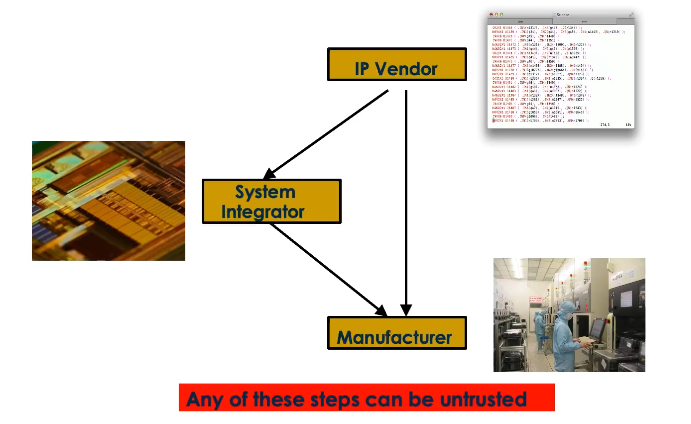
\includegraphics[width=0.7\textwidth]{img/hardware/supply chain.png}
    \caption{The hardware threat model}
  \end{figure}
  As a consequence, none of the companies involved in the process can be trusted, but they were,
  that being why so many security issues are being discovered nowadays.\\
  The modern approach is kind of different, because designing the chip and outsourcing the manufacturing process is 
  so prone to security issues, the hardware, or its description, is simply bought from a trusted 
  source.\\
  The threat is still there, but it is reduced and independent from the company that is actually
  implementing the hardware. Sometimes the cheapest solution is just to accept the risk.\\

  \begin{figure}[H]
    \centering
    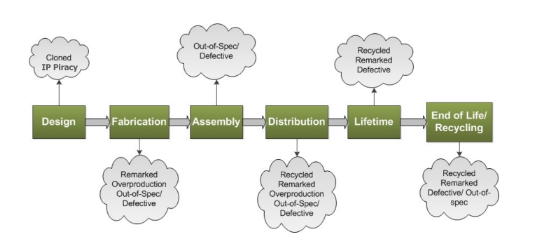
\includegraphics[width=0.8\textwidth]{img/hardware/supply chain vulnerabilies.png}
    \caption{The supply chain vulnerabilities of hardware}
  \end{figure}
\end{section}
\begin{section}{Background on security}
  First of all, the whole point of security is to deal with \textbf{threats}, which are the actions
  that could cause harm to an asset by exploiting a vulnerability(a \textit{weakness} of a system), 
  and \textbf{risk}, which is a qualitative or quantitative measurement of the probability of  
  security event and its impact.\\
  A few other things to recall are that an attack is a deliberate action to exploit a vulnerability,
  and the attack surface is the sum of all the possible risk exposures of a system.\\
  \begin{boxH}
    \textbf{Hardware security} deals with sensitive assets, such as cryptographic keys, in the 
    hardware from malicious physical, software and network attacks and provides the appropriate 
    level of isolation between secure and non-secure data code, in addition to supplying separation
    between multiple user applications.
  \end{boxH}
  This is easier said than done, because the informations needs to be secure both from the architectural
  point of view(cpu, memory, etc) and the micro-architectural point of view, which is the actual
  implementation of the architecture.\\
  And because the micro-architecture is very complex, unexpected behaviors are to be expected, and
  can be exploited by an attacker.\\
  Furthermore, because hardware and software are so intertwined, sometimes hardware vulnerabilities
  can be exploited by software code.\\

  \begin{figure}[H]
    \centering
    \subfloat[Architecture of a Intel Skylake processor]{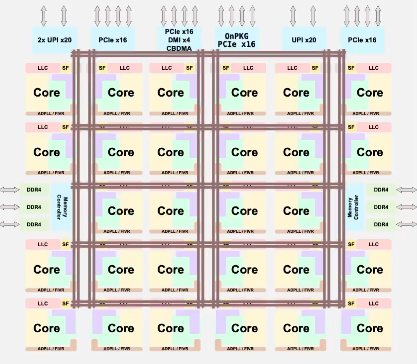
\includegraphics[width=0.4\textwidth]{img/hardware/skylake architecture.png}}
    \hfill
    \subfloat[Micro-architecture of a core of Intel Skylake processor]{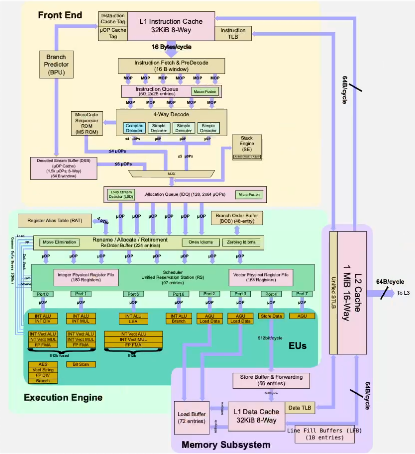
\includegraphics[width=0.4\textwidth]{img/hardware/skylake micro-architecture.png}}
  \end{figure}
  That being said, the typical approach to security in general is predict possible breaches and 
  vulnerabilities, and then try to prevent them, either by identifying them of waiting for them to
  be discovered.\\
  \begin{subsection}{Hardware security and trust}
    As previously explained, hardware security is a very broad field, that covers both the security
    of the hardware itself but also the trustworthiness of the hardware.\\
    You can see from figure \ref{fig:hardware security fields} that this field can be split in different 
    categories and subcategories.\\

    \begin{figure}[h]
      \centering
      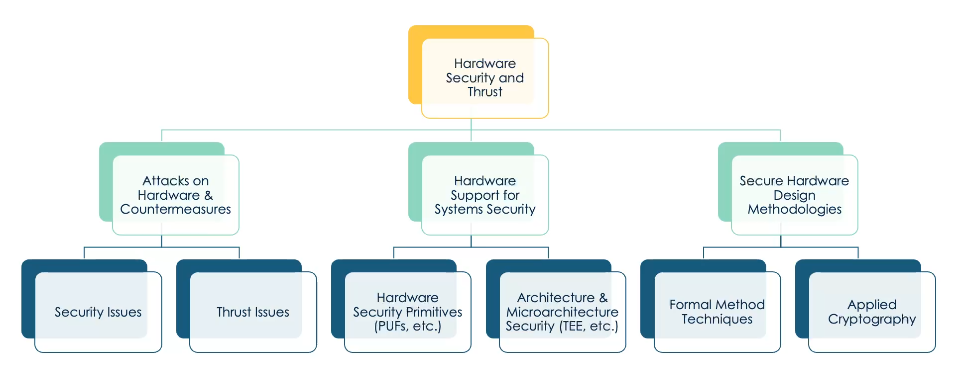
\includegraphics[width=0.9\textwidth]{img/hardware/hardware security schema.png}
      \caption{General schema of hardware security and trust fields}
      \label{fig:hardware security fields}
    \end{figure}
    At first, it covers \textbf{security issues}, \textbf{trust issues}(checking if the hardware
    is what it is supposed to be) and the possible countermeasures.\\
    Then, it covers the \textbf{supporting technologies} to the system security, such as security
    primitives(true number generators as such) and means to execute code in a secure way(as trusted
    execution environments).\\
    Finally, it covers the \textbf{design methodologies} to ensure the security of the hardware, such
    as the use of formal methods, the use of secure hardware description languages and secure hardware design flows.
  \end{subsection}
\end{section}
\begin{section}{Hardware vulnerabilities}
  When we are talking about hardware vulnerabilities, some of the most common are:
  \begin{itemize}
    \item \textbf{Physical attacks}: also called \textit{fault injection attacks}
    \item \textbf{Trojans Horses}
    \item \textbf{IP Piracy}
    \item \textbf{IC Piracy and Counterfeiting}
    \item \textbf{Backdoors}
    \item \textbf{Tampering}: changing the hardware to make it behave differently
    \item \textbf{Reverse Engineering}: its not a defect, but can cause a monetary loss
    \item \textbf{Functional Bugs}
    \item \textbf{Side-Channel Bugs}
  \end{itemize}
\end{section}
\begin{section}{Hardware Controls for Secure Systems}
  The goal of hardware controls is to ensure that the hardware is secure and trustworthy, and to
  that end, some controls are needed.\\
  \begin{itemize}
    \item Hardware implementations of encryption
    \item Encryption has to do with scrambling to hide
    \item Design locks or physical locks limiting access
    \item Devices to verify the user identities
    \item Hiding signatures in the design files
    \item Intrusion detection
    \item Hardware boards limiting memory access
    \item Tamper-resistant
    \item Policies and procedures
    \item $\dots$
  \end{itemize}
  The list can go on and on, but the point is that security processes add overhead to the system,
  lowering its power efficiency and performance.\\
  This can be a huge deal when working with system with strict power and performance requirements,
  such as embedded systems.\\
  Security has become a new design challenge that must be considered at the design time, along with 
  other metrics, i.e., cost, power, area.
\end{section}

